%!TEX root = ../thesis_a4.tex

\chapter{Appendix A: Freesound}
\label{appendix:Freesound}

\section{Introduction}
\label{appendix:Freesound_intro}

Freesound is an online sharing platform where people with diverse interests share recorded sound samples under Creative Commons licenses (Fig.~\ref{fig:app:screenshot}). 
The audio content that can be shared in Freesound is restricted to \emph{sounds}, which may include any kind of audio material like sound effects, environmental recordings or even building blocks for musical compositions, but not music tracks in the traditional sense of ``finished'' compositions or songs.
It was started in 2005 at the Music Technology Group\footnote{\url{http://mtg.upf.edu}} of Universitat Pompeu Fabra, and it is being maintained to support diverse research projects and as a service to the overall research and artistic community. 
Freesound's initial goal was to give support to sound researchers, who often have trouble finding large royalty-free sound databases to test their algorithms, and to sound artists, who use pre-recorded sounds in their pieces. After eight years since its inception, Freesound has become one of the most popular sites for sharing sound samples, with an average of 45,000 unique visitors per day.
More importantly, there is a highly engaged community of users continuously contributing to the site, not only uploading sounds but also commenting, rating and discussing in the forums about relevant topics for the community.
All sounds in Freesound are manually moderated by a group of Freesound users (the Freesound moderators) that check for the accurateness of sound annotations and for adequacy of uploaded sounds.

\begin{figure}
 \centerline{
 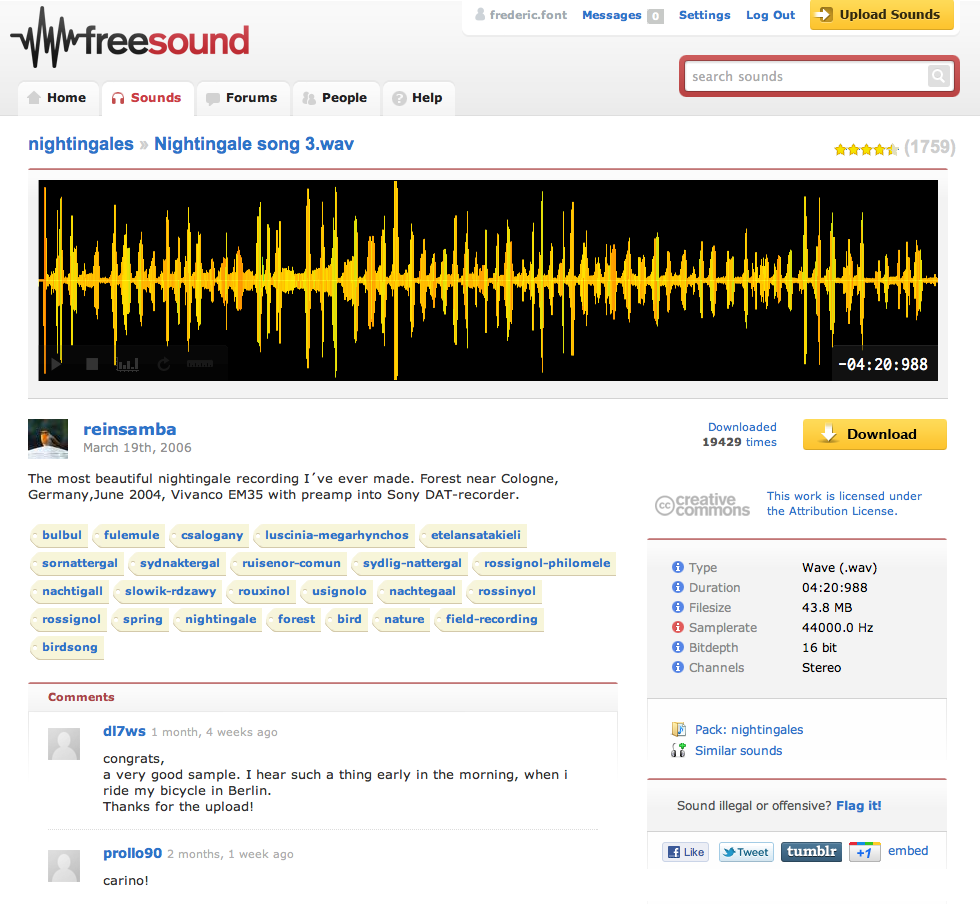
\includegraphics[width=0.8\columnwidth]{ch99/pics/freesound_screenshot.png}}
 \caption{Screenshot of a sound page of Freesound.}
 \label{fig:app:screenshot}
\end{figure}

All the content in Freesound is released under Creative Commons licenses. When uploading sounds, Freesound users can choose between CC0 (public domain), Attribution and Attri\-bu\-tion-NonCommercial licences\footnote{\url{http://www.creativecommons.org/licenses}}. The reason to offer these licenses is to ensure that all the content uploaded in Freesound can be reused by other users, developers and researchers, but at the same time we provide users the option to require the attribution of their work or to restrict the use of their sounds to non-commercial activities. Furthermore, the source code of the web application is released as open source\footnote{\url{http://www.github.com/MTG/freesound}} under the GNU AGPL license\footnote{\url{http://www.gnu.org/licenses/agpl.html}}.

\begin{figure}
 \centerline{
 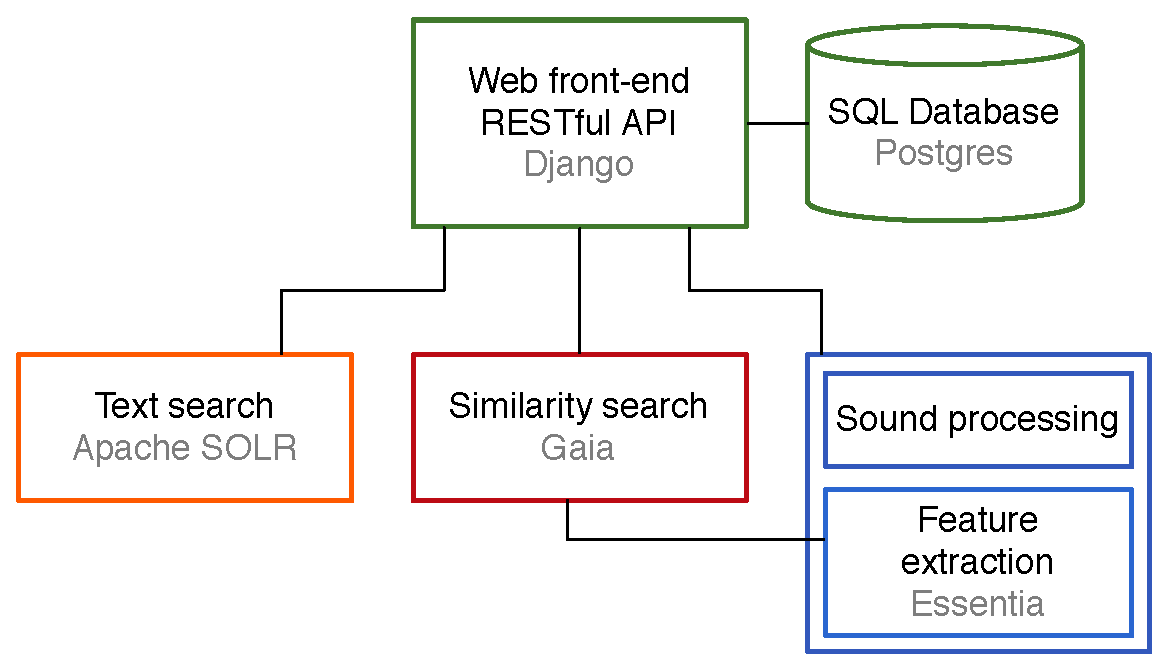
\includegraphics[width=0.7\columnwidth]{ch99/pics/architecture.eps}}
 \caption{Simplified diagram of the Freesound architecture~\citep{Font2013b}.}
 \label{fig:app:architecture}
\end{figure}

Freesound was built with high load and scalability in mind. 
Fig.~\ref{fig:app:architecture} shows a block diagram of its architecture. 
Retrieval of sounds can be performed using text queries, audio content-based similarity search, or by browsing tags or geotags. 
Content-based similarity search is performed over a broad set of low-level audio features\footnote{A list of these features can be found here: \url{http://www.freesound.org/apiv2/descriptors/} (requires Freesound account).}, extracted with Essentia\footnote{\url{http://essentia.upf.edu}}~\citep{Bogdanov2013}, an open-source audio feature extraction tool also developed at the Music Technology Group, and indexed in Gaia\footnote{\url{http://github.com/mtg/gaia}}, another open-source tool developed at the Music Technology Group to build and query large feature spaces.
The front-end is a Django\footnote{\url{http://www.djangoproject.com}} application which includes basic social interaction features (forum, sound comments, sound ratings, private messaging, etc.), and using a PostgreSQL\footnote{\url{http://www.postgresql.org}} database for permanent storage.
Text indexing is supported by an Apache Solr\footnote{\url{http://lucene.apache.org/solr}} server including text descriptions and tags, which allows for sophisticated text queries using the Solr query syntax. 
A distributed architecture is used for processing incoming sounds, producing compressed previews and waveform/spectrogram images, as well as for audio feature extraction. Frame-level and sound-level features are available for each sound.

In 2011, a major update to Freesound was deployed which included a complete redesign of both the backend and the frontend the site, and introduced an API to facilitate access to the Freesound content to researchers and developers\footnote{\url{http://www.freesound.org/docs/api/}}. The API runs as a Django application based on the RESTful principles. 
With the Freesound API users can browse, search, and retrieve information about Freesound users, packs, and the sounds themselves, and also upload, comment, rate and bookmark sounds. 
Furthermore, the API allows to search for similar sounds to a given target (based on audio content features) and to retrieve content features extracted from the audio files, as well as to perform advanced queries combining content analysis features and other metadata such as tags and textual descriptions. 

In the following sections we briefly describe some information about Freeound which can be of interest to the reader of this thesis.
First, we provide statistics about some aspects of general interest. % (Sec.~\ref{sec:app:freeosund_gen_numbers}).
Then, we provide further insight into the community of users around Freesound. % (Sec.~\ref{sec:app:survey}).
For further information we refer the reader to previous publications by the authors~\citep{Font2012,Font,Font2013b}.

\section{General numbers}
\label{sec:app:freeosund_gen_numbers}

\begin{table}
\begin{threeparttable}
\ra{1.2}
\footnotesize
  \begin{center}
    \makebox[0pt]{
    \begin{tabular}{@{}lr@{\hskip 1.0cm}lr@{}} %
      \toprule
      Number of sounds 	& 						230,327  	&  Number of contributor users\tnote{a} & 		14,353  \\
      Number of sound packs &					14,004 	 	&  Number of unique tags\tnote{b} & 			77,753 \\ 
      Number of sound comments & 				191,556 	&  Number of tag applications 	& 				1,670,159	\\
      Number of sound ratings &  				929,380 	&  Average number of tags per sound & 			7.19 	\\ % 5.233 std
      Number of sound downloads & 				65,399,428  &  Number of forum posts & 						47,350 \\  
      Number of registered users & 				4,341,738   &  Number of forum threads & 					9,648 \\
      
      \bottomrule
    \end{tabular}
  }
    \begin{tablenotes}
    \item[a] Users that have contributed by uploading, at least, one sound.
    \item[b] Not necessarily semantically unique.
    \end{tablenotes}
  \caption[Basic statistics of Freesound]{Basic statistics of Freesound (at the time of this writing).}
  \label{app:tab:fs_stats}
  \end{center}
\end{threeparttable}
\end{table}

\begin{figure}
\centerline{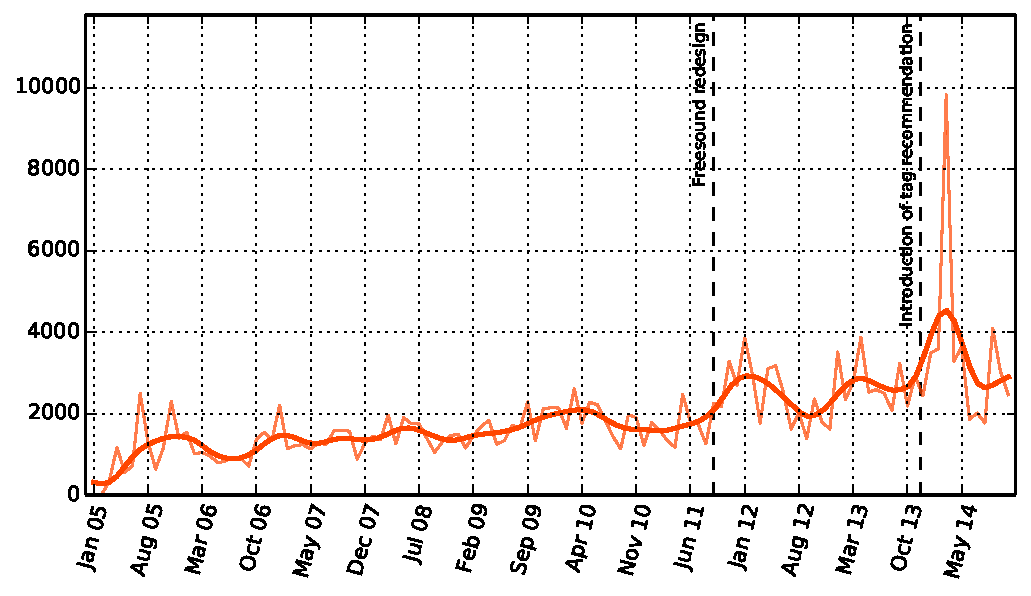
\includegraphics[width=1.0\columnwidth]{ch99/pics/Number_of_sounds}}
\caption[Evolution of the number of sounds]{Evolution of the number of uploaded sounds per month. The stronger line corresponds to a smoothed version of the number of uploaded sounds, using a Hann window of 11 points.}
\label{app:fs:new_sounds}
\end{figure}

\begin{figure}
\centerline{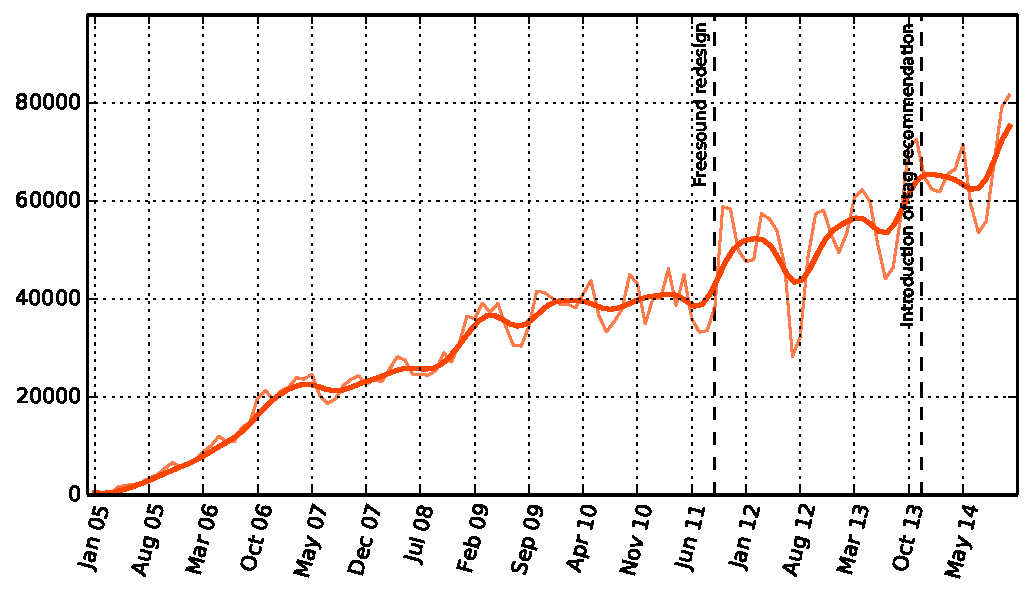
\includegraphics[width=1.0\columnwidth]{ch99/pics/Number_of_users}}
\caption[Evolution of the number of newly registered users]{Evolution of the number of newly registered users per month. The stronger line corresponds to a smoothed version of the number of newly registered users, using a Hann window of 11 points.}
\label{app:fs:new_users}
\end{figure}


In Table \ref{app:tab:fs_stats} we report some numbers of general interest about several Freesound aspects such as the number of sounds, users, tags and the distinct social activities.
Figs.~\ref{app:fs:new_sounds},~\ref{app:fs:new_users} and~\ref{app:fs:new_tags} complement these numbers by showing the evolution of the number of uploaded sounds, newly registered users, and new tags per month.
It is particularly interesting to observe that both the number of uploaded sounds and newly registered users per month has been steadily increasing since the start of Freesound in 2005.
Furthermore, it is interesting to note the sudden increase in the number of new tags per month that happened along with the aforementioned redesign of Freesound (Sec.~~\ref{appendix:Freesound_intro}) and the later decrease after the introduction of the tag recommendation system (Fig.~\ref{app:fs:new_tags}).
This evolution suggests that the new Freesound design had a huge impact on the way users annotate sounds, resulting in less reuse of tags. This might be explained because, before the redesign, Freesound's annotation interface included a section in which the most commonly used tags by someone annotating a sound were shown. This section was removed after the redesign.
After the introduction of tag recommendation however, the rate at which new tags are created diminishes, as we already observed and discussed in Chapter~\ref{sec:impact} (Sec.~\ref{impact:sec:percentage_of_new_tags_results}) and can also be seen in Fig.~\ref{app:fs:new_tags}.


\begin{figure}
\centerline{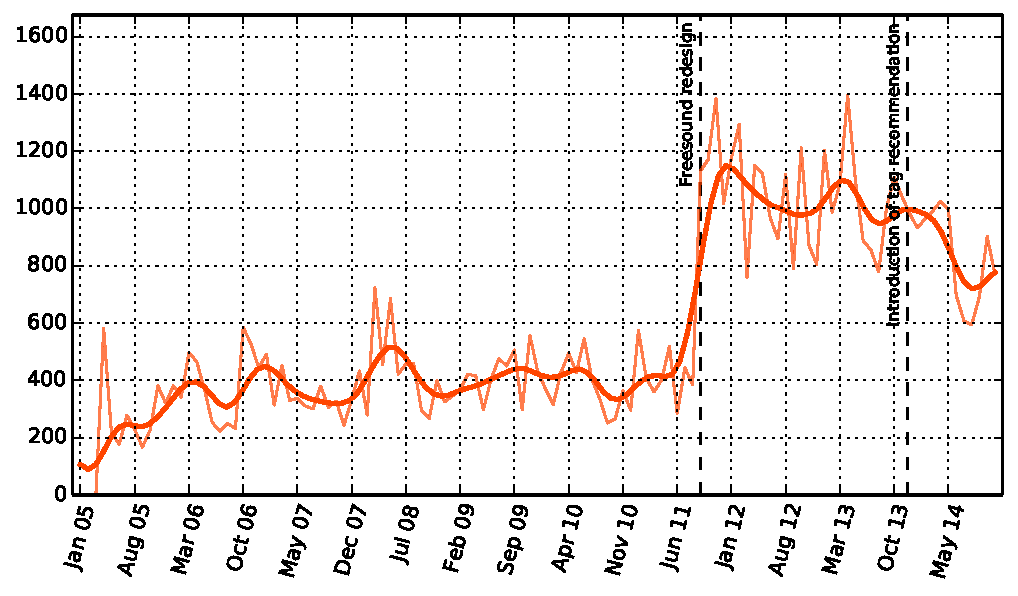
\includegraphics[width=1.0\columnwidth]{ch99/pics/Number_of_new_tags}}
\caption[Evolution of the number of new tags]{Evolution of the number of new tags per month. The stronger line corresponds to a smoothed version of the number of new tags, using a Hann window of 11 points.}
\label{app:fs:new_tags}
\end{figure}


%\begin{figure}
%\centerline{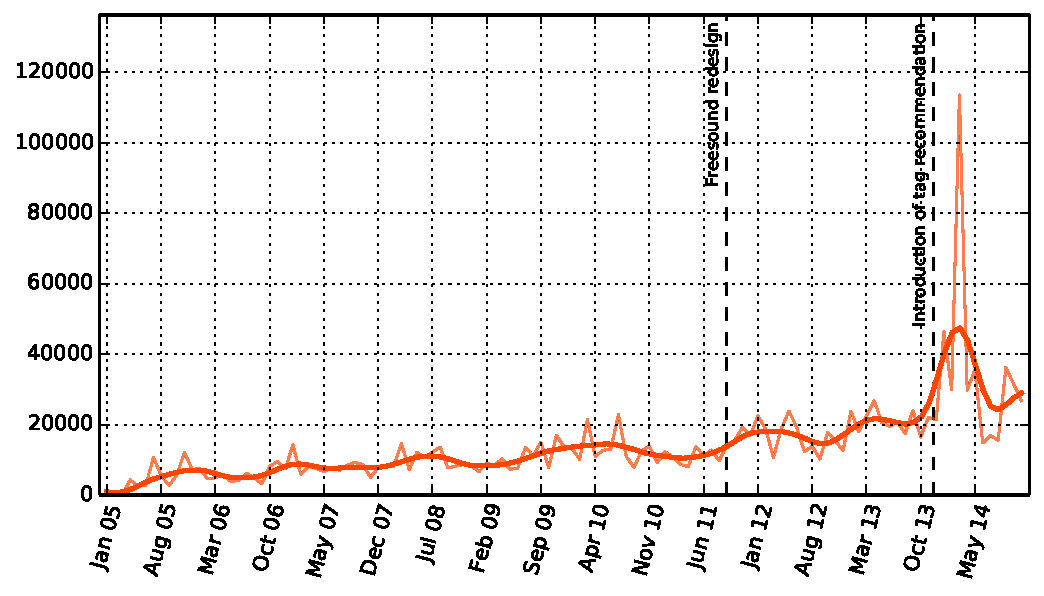
\includegraphics[width=\figSizeMidLarge]{ch99/pics/Number_of_tag_applications}}
%\caption[Evolution of the number of new tag applications]{Evolution of the number of new tag applications per month. The stronger line corresponds to a smoothed version of the number of new tag applications, using a Hann window of 11 points.}
%\label{app:fs:new_tag_applications}
%\end{figure}


\section{Freesound's community of users}
\label{sec:app:survey}

%The active contributors in the community have played an important role in the development of the platform, since quite a number of the software improvements have been the result of suggestions from the community or have been discussed within it. Two basic goals have driven most of the development of Freesound: quality and quantity of sounds. We wanted to gather as many user contributed sounds as possible, but not at any price. Sounds have to be of good quality and have to be well described in order to be easily found and reused.

The active community of users behind Freesound is the clearest indication of its success.
As we have already seen, the community has been growing over time, reaching more than 4 million registered users and 14,000 unique sound contributors at the time of this writing.
Freesound's community can be characterised as a ``task-oriented'' community, that is to say, a community where its members pursue some collective goals that benefit the whole community~\citep{Stanoevska-slabeva2002a}. 
To get some insight in that aspect, we carried out a small online survey in the Freesound forums, asking users about their opinion on the existence of shared goals and, if so, which are these goals.
A total of 86 Freesound users participated in the survey, 50 of them agreeing with the existence of shared goals, and the others either not directly answering the question (31) or denying the existence of these goals (5).
Shared goals that users described in their responses are quite diverse. However, the most repeated goals could be summarized as ``sharing sounds'' (mentioned by 43\% of those participants agreeing with the existence of shared goals), ``building a big sound archive'' (30\%) and ``helping each other by uploading useful sounds'' (21\%).

Furthermore, in that same survey we also asked users about the things that make Freesound different from other similar sites. In that case, 66\% of users pointed either at the quantity, quality, diversity or ``freeness'' of accessible sounds, all of them being primary design criteria for Freesound. Other common answers are related to the user interface or the focus on sharing sound samples rather than music (24\% of the responses). 

Finally, we asked users about the applications for which Freesound is being used (i.e.,~for what purposes Freesound samples are being reused). 
Responses show that the most important usage of Freesound samples is in movies and animations (35\%), followed by music (20\%), theatre (9\%), sound design (9\%), education and academy (6\%), and videogames (5\%). Particularly interesting is the fact that the remaining 16\% of users pointed out Freesound itself as an application, and hence mainly using Freesound for listening, sharing and contributing sounds, and for its basic social functionalities.
 